\documentclass[12pt]{report}
\usepackage{graphicx}     %standard package. Note graphics<graphicx<epsfig
%\usepackage{color}     %standard package
\usepackage[colorlinks]{hyperref} %standard package written by Sebastian Rahtz
%\usepackage{subeqn}    %allows equations 1a, 1b
%\usepackage{subfig}    %allows figures 1a, 1b
\usepackage{amsmath}
\usepackage{amssymb}
\usepackage{url} 
\usepackage[sorting=none]{biblatex}
\addbibresource{references.bib}

\paperheight=11in
\topmargin=0in
\headheight=0in
\headsep=0in
\topskip=0in
\textheight=8.5in
\footskip=.5in

\paperwidth=8.5in
\oddsidemargin=0in
\evensidemargin=0in
\textwidth=7.0in
\parindent=.5in

\newtheorem{claim}{Claim}
\newcommand{\proof}[0]{{\bf proof:} }
\newcommand{\qed}[0]{\newline\noindent{\bf QED }}


\newcommand{\bra}[1]{\langle#1|}
\newcommand{\ket}[1]{|#1\rangle}
\newcommand{\av}[1]{\langle#1\rangle}
\newcommand{\pder}[2]{\frac{\partial#1}{\partial#2}}
\newcommand{\tr}[0]{{\rm tr }}
\newcommand{\beq}{\begin{equation}}
\newcommand{\eeq}{\end{equation}}
\newcommand{\bsub}{\begin{subequations}}
	\newcommand{\esub}{\end{subequations}}
\newcommand{\beqa}{\begin{eqnarray}}
\newcommand{\eeqa}{\end{eqnarray}}
\newcommand{\rarrow}[0]{\rightarrow}
\newcommand{\larrow}[0]{\leftarrow}
\newcommand{\Rarrow}[0]{\Rightarrow}
\newcommand{\nRarrow}[0]{\nRightarrow}
\newcommand{\Larrow}[0]{\Leftarrow}
\newcommand{\nLarrow}[0]{\nLeftarrow}
\newcommand{\ul}[1]{\underline{#1}}
\newcommand{\ol}[1]{\overline{#1}}
\newcommand{\ZZ}[0]{ {\mathbb{Z}}}
\newcommand{\RR}[0]{{ \mathbb{R}} }
\newcommand{\CC}[0]{{ \mathbb{C}} }
\newcommand{\ground}{{}_{\stackrel{\stackrel{\displaystyle{\bot}}{-}}{.}}}


\newcommand{\rva}[0]{{\ul{a}}}
\newcommand{\rvb}[0]{{\ul{b}}}
\newcommand{\rvc}[0]{{\ul{c}}}
\newcommand{\rvd}[0]{{\ul{d}}}
\newcommand{\rve}[0]{{\ul{e}}}
\newcommand{\rvf}[0]{{\ul{f}}}
\newcommand{\rvg}[0]{{\ul{g}}}
\newcommand{\rvh}[0]{{\ul{h}}}
\newcommand{\rvi}[0]{{\ul{i}}}
\newcommand{\rvj}[0]{{\ul{j}}}
\newcommand{\rvk}[0]{{\ul{k}}}
\newcommand{\rvl}[0]{{\ul{l}}}
\newcommand{\rvm}[0]{{\ul{m}}}
\newcommand{\rvn}[0]{{\ul{n}}}
\newcommand{\rvo}[0]{{\ul{o}}}
\newcommand{\rvp}[0]{{\ul{p}}}
\newcommand{\rvq}[0]{{\ul{q}}}
\newcommand{\rvr}[0]{{\ul{r}}}
\newcommand{\rvs}[0]{{\ul{s}}}
\newcommand{\rvt}[0]{{\ul{t}}}
\newcommand{\rvu}[0]{{\ul{u}}}
\newcommand{\rvv}[0]{{\ul{v}}}
\newcommand{\rvw}[0]{{\ul{w}}}
\newcommand{\rvx}[0]{{\ul{x}}}
\newcommand{\rvy}[0]{{\ul{y}}}
\newcommand{\rvz}[0]{{\ul{z}}}

\newcommand{\rvX}[0]{{\ul{X}}}
\newcommand{\rvY}[0]{{\ul{Y}}}
\newcommand{\rvZ}[0]{{\ul{Z}}}

\newcommand{\rvA}[0]{{\ul{A}}}
\newcommand{\rvB}[0]{{\ul{B}}}
\newcommand{\rvC}[0]{{\ul{C}}}
\newcommand{\rvD}[0]{{\ul{D}}}


\newcommand{\cala}[0]{{\cal A}}
\newcommand{\calb}[0]{{\cal B}}
\newcommand{\calc}[0]{{\cal C}}
\newcommand{\cald}[0]{{\cal D}}
\newcommand{\cale}[0]{{\cal E}}
\newcommand{\calg}[0]{{\cal G}}
\newcommand{\calh}[0]{{\cal H}}
\newcommand{\cali}[0]{{\cal I}}
\newcommand{\call}[0]{{\cal L}}
\newcommand{\caln}[0]{{\cal N}}
\newcommand{\calp}[0]{{\cal P}}
\newcommand{\cals}[0]{{\cal S}}
\newcommand{\calt}[0]{{\cal T}}
\newcommand{\calu}[0]{{\cal U}}
\newcommand{\calv}[0]{{\cal V}}


\newcommand{\lam}[0]{\lambda}
\newcommand{\indi}[0]{\hat{1}}
\newcommand{\pp}[0]{\mathbb{P}}
\newcommand{\dbm}[0]{{
		[1,\partial_{b},\partial_{m}]
}}

\newcommand{\dg}[0]{{[1, \partial_{\theta_G}]}}
\newcommand{\dd}[0]{{[1, \partial_{\theta_D}]}}
\newcommand{\dgd}[0]{{[1, \partial_{\theta_G}, \partial_{\theta_D}]}}

\newcommand{\vecc}[0]{{\vec{c}}}
\newcommand{\vecd}[0]{{\vec{d}}}
\newcommand{\vecf}[0]{{\vec{f}}}
\newcommand{\vecr}[0]{{\vec{r}}}
\newcommand{\vecu}[0]{{\vec{u}}}
\newcommand{\vecx}[0]{{\vec{x}}}
\newcommand{\vecy}[0]{{\vec{y}}}
\newcommand{\vechy}[0]{{\vec{\hat{y}}}}
\newcommand{\vtheta}[0]{{\vec{\theta}}}

%\includeonly{gan/gan}

\begin{document}
\title{\textbf{Bayesuvius}, \\a small visual dictionary of Bayesian Networks}



\author{Robert R. Tucci\\
        www.ar-tiste.xyz}

\date{ \today}

\maketitle

\begin{figure}[h!]
\centering
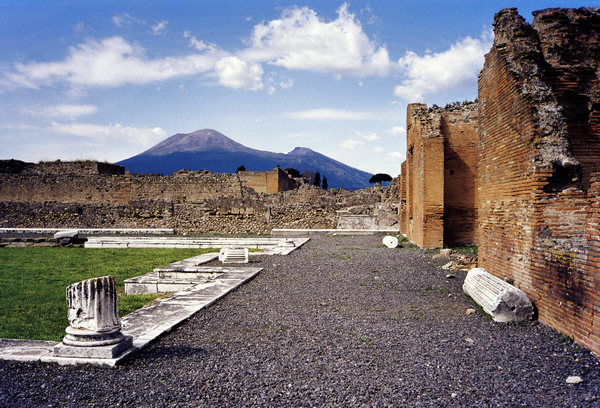
\includegraphics[width=6.5in]{vesuvius-from-pompei.png}
\caption{View of Mount Vesuvius from  Pompeii} 
\end{figure}

\newpage
\tableofcontents
\section{Foreword}
Welcome to Bayesuvius! a proto-book uploaded to github.

A different Bayesian network is discussed in each chapter. Each chapter title is the name of a B net. Chapter titles are in alphabetical order.

This is a volcano in its early stages. First version uploaded to a github repo called Bayesuvius on June 24, 2020. First version only covers 2 B nets (Linear Regression and GAN). I will add more chapters periodically. Remember, this is a moonlighting effort so I can't do it all at once.

For any questions about notation, please go to Notational Conventions section.

Requests and advice are welcomed.


\bigskip
\noindent Thanks for reading this.

\noindent Robert R. Tucci

\noindent www.ar-tiste.xyz

\section{Notational Conventions}
\hrule
bnet=B net=Bayesian Network
\hrule

Random Variables will be indicated by underlined letters and their values by non-underlined letters. Each node of a bnet will be labelled by a random variable. Thus, $\rvx=x$ means that node $\rvx$ is in state $x$.
\smallskip
\hrule
 $P_\rvx(x)=P(\rvx=x)=P(x)$ is the probability that random variable $\rvx$ equals $x\in S_\rvx$. $S_\rvx$ is the set of states (i.e., values) that $\rvx$ can assume and $n_\rvx = |S_\rvx|$ is the size (aka cardinality) of that set. Hence, 
\beq
\sum_{x\in S_\rvx}P_\rvx(x)=1
\eeq
\hrule
\beq
P_{\rvx,\rvy}(x,y)=P(\rvx=x, \rvy=y)=P(x,y)
\eeq
\beq
P_{\rvx|\rvy}(x|y)=P(\rvx=x| \rvy=y)=P(x|y)=\frac{P(x,y)}{P(y)}
\eeq
\hrule
Kronecker delta function: For $x,y$ in discrete set $S$, 
\beq
\delta(x,y)=\left\{
\begin{array}{l}
1\;{\rm if}\; x=y
\\
0 \;{\rm if}\; x\neq y
\end{array}
\right.
\eeq
\hrule
Dirac delta function: For $x,y\in\RR$,
\beq
\int^{+\infty}_{-\infty}dx\;\delta(x-y)f(x)=f(y)
\eeq
\hrule
Indicator function:
\beq
\indi(\cals)=\left\{
\begin{array}{l}
1\;{\rm if\; \cals\; is\; true} 
\\
0 \;{\rm if \;\cals\; is \;false}
\end{array}
\right.
\eeq
For example, $\delta(x,y)=\indi(x=y)$.
\hrule
\beq
\vec{x}= (x[0], x[1], x[2] \ldots, x[nsam(\vecx)-1])=x[:]
\eeq

 $nsam(\vecx)$ is the number of samples  of $\vecx$. $\rvx[i]$ are i.d.d. (independent identically distributed) samples with

 \beq
x[i]\sim P_\rvx\;\;({\rm i.e.}\; P_{\ul{x[i]}}=P_\rvx)
\eeq

\beq
P(\rvx=x)=\frac{1}{nsam(\vecx)}\sum_i \indi(x[i]=x)
\eeq 

If we use two sampled variables, say $\vecx$ and $\vecy$, in a given bnet, their number of samples $nsam(\vecx)$ and $nsam(\vecy)$ need not be equal.
\hrule
\beq
P(\vecx) = \prod_i P(x[i])
\eeq

\beq
\sum_\vecx = \prod_i\sum_{x[i]}
\eeq

\beq
\partial_\vecx = 
[\partial_{x[0]}, \partial_{x[1]},\partial_{x[2]}, \dots, \partial_{x[nsam(\vecx)-1]}]
\eeq
\hrule 
\beqa
P(\vecx)&\approx& [\prod_x P(x)^{P(x)}]^{nsam(\vecx)} \\
&=& e^{nsam(\vecx)\sum_x P(x)\log P(x)}\\
&=& e^{-nsam(\vecx)H(P_\rvx)}
\eeqa

\hrule 

\beq
f^{[1, \partial_x, \partial_y]}(x,y) =
[f, \partial_x f , \partial_y f]
\eeq

\beq
f^+=
f^{[1, \partial_x, \partial_y]}
\eeq
\hrule
For probabilty distributions $p(x), q(x)$ of $x\in S_\rvx$
\begin{itemize}
\item 
Entropy:
\beq
H(p)=-\sum_x p(x)\log p(x)\geq 0
\eeq

\item
Kullback-Liebler divergence:

\beq
D_{KL}(p\parallel q)=\sum_{x} p(x)\log \frac{p(x)}{q(x)}\geq 0
\eeq
\item 
Cross entropy:
\beqa
CE(p\rarrow q) &=& -\sum_x p(x)\log q(x)\\
&=& H(p) + D_{KL}(p\parallel q)
\eeqa
\end{itemize}

\hrule
Normal Distribution: $x, \mu, \sigma\in \RR$, $\sigma >0$

\beq 
\caln(\mu, \sigma)(x)=
\frac{1}{\sigma\sqrt{2\pi}}
e^{-\frac{1}{2}\left(
\frac{x-\mu}{\sigma}\right)^2}
\eeq
\hrule
Uniform Distribution: $a<b$, $x\in [a,b]$

\beq
\calu(a,b)(x) =
\frac{1}{b-a}
\eeq
\chapter{Generative Adversarial Network (GAN)}
%\begin{refsection}

\begin{figure}[h!]
\centering
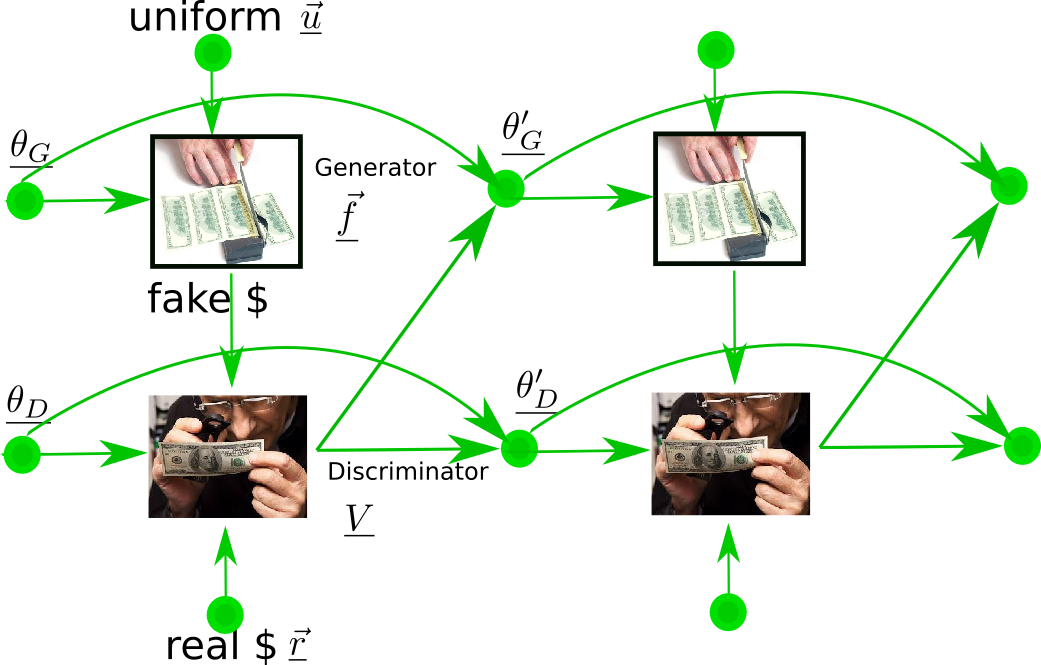
\includegraphics[width=6in]{gan/gan.png}
\caption{Generative Adversarial  Network (GAN)} 
\label{fig-gan}
\end{figure}

\begin{figure}[h!]
\centering
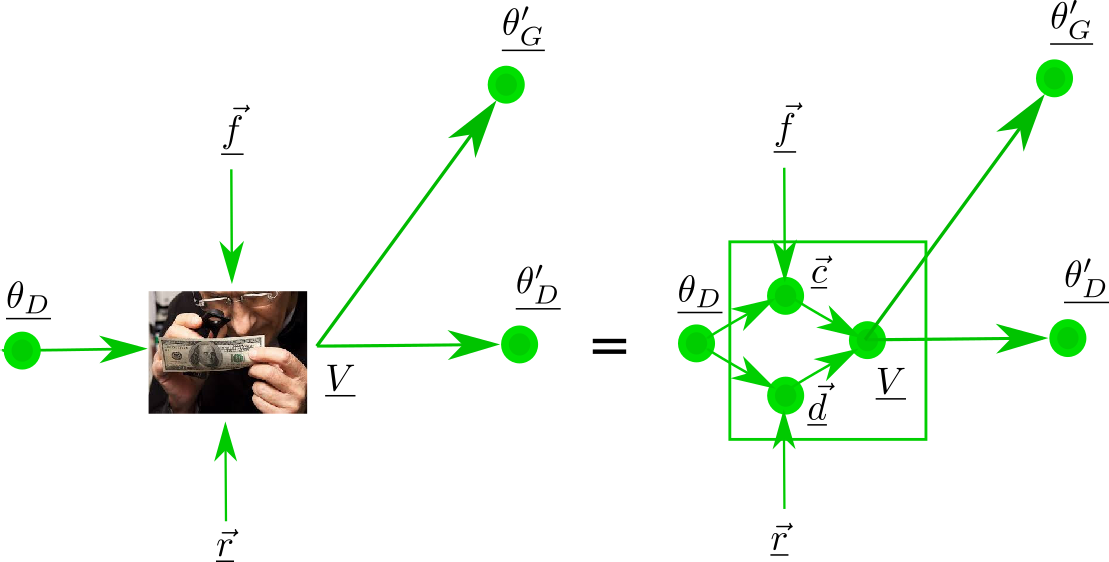
\includegraphics[width=6in]{gan/gan-detail.png}
\caption{Discriminator node $\ul{V}$ in Fig.\ref{fig-gan} can be
split into 3 nodes $\vec{\rvc}$, $\vec{\rvd}$ and $\ul{V}$.} 
\label{fig-gan-detail}
\end{figure}

Original GAN, 
Ref.\cite{gf2014}(2014). 

Generator $G$ (counterfeiter) generates samples $\vecf$ of fake money and submits them to Discriminator $D$ (Treasury agent). $D$ also gets samples $\vecr$ of real money. $D$ submits veredict $V\in [0,1]$. $G$ depends on parameter $\theta_G$ and $D$ on parameter $\theta_D$. Veredict $V$ and initial $\theta_G, \theta_D$ are used to get new parameters $\theta'_G, \theta'_D$.Process is repeated (Dynamical Bayesian Network) until saddle point in $V(\theta_G, \theta_D)$ is reached. $D$ makes $G$ better and vice versa.  Zero-sum game between $D$ and $G$.



Let $\cald$ be the domain of $D(\cdot, \theta_D)$. Assume that for any $x\in \cald$,

\beq
0\leq D(x,\theta_D)\leq 1
\;.
\eeq
For any $S\subset\cald$, define

\beq
\sum_{x\in S}D(x,\theta_D)=\lam(S,\theta_D)
\;.
\eeq


 In general, 
$G(\cdot,\theta_G)$ need not be real valued. 

Assume that for every $u\in S_\rvu$,
 $G(u,\theta_G)=f\in S_\rvf\subset \cald$. Define
\beq
\ol{D}(f,\theta_D)=1-D(f,\theta_D)
\;.
\eeq
Note that

\beq
0\leq\ol{D}(f,\theta_D)\leq 1
\;.
\eeq

Define:

\beq
V(\theta_G, \theta_D) =
\sum_{r}P(r)
\log D(r, \theta_D)
+ \sum_{u}P(u)\log
\ol{D}(G(u,\theta_G),\theta_D)
\;.	
\eeq

We want the first variation of $V(\theta_G, \theta_D)$ to vanish.




\beq
\delta V(\theta_G, \theta_D)=0
\;.
\eeq
This implies

\beq
 \partial_{\theta_G}V(\theta_G, \theta_D)=
 \partial_{\theta_D}V(\theta_G, \theta_D)=0
\;
\eeq
and

\beq
V_{opt}=\min_{\theta_G}\max_{\theta_D} V(\theta_G, \theta_D)
\;.
\eeq

Node transition  probability matrices
for Figs.\ref{fig-gan} and \ref{fig-gan-detail} 
are
given next in blue:

\beq\color{blue}
P(\theta_G)=\;{\rm given}
\eeq

\beq\color{blue}
P(\theta_D)=\;{\rm given}
\eeq


\beq\color{blue}
P(\vecu)=\prod_i P(u[i])  \;\;{\rm (usually \;uniform\; distribution)}
\eeq

\beq\color{blue}
P(\vecr)=\prod_i P(r[i])
\eeq


\beq\color{blue}
P(f[i]|\vecu, \theta_G)= \delta[f[i], G(u[i],\theta_G)]
\eeq

\beq\color{blue}
P(c[i]|\vecf, \theta_D) = \delta(c[i], \ol{D}(f[i], \theta_D))
\eeq

\beq\color{blue}
P(d[j]|\vecr, \theta_D)= \delta(d[j], D(r[j], \theta_D))
\eeq




\beq\color{blue}
P(V| \vecd,  \vecc)=
\delta(V, \frac{1}{N}\log \prod_{i,j}(c[i]d[j]))
\eeq
where $N=nsam(\vecr)nsam(\vecu)$.







Let $\eta_G, \eta_D> 0$. Maximize $V$ wrt $\theta_D$, and
minimize it wrt $\theta_G$.

\beq\color{blue}
P(\theta'_G|V,\theta_G )=
\delta(\theta'_G, \theta_G - \eta_G 
\partial_{\theta_G}V)
\eeq

\beq\color{blue}
P(\theta'_D|V,\theta_D )=
\delta(\theta'_D, \theta_D + \eta_D 
\partial_{\theta_D}V)
\eeq

\hrule
\begin{figure}[h!]
\centering
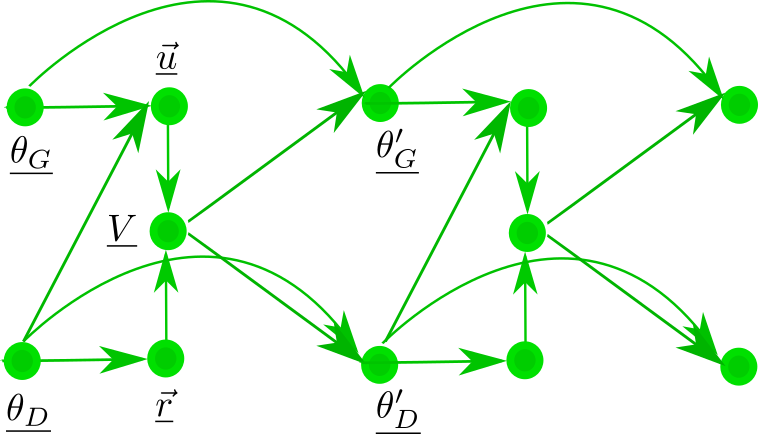
\includegraphics[width=2in]{gan/gan-emulate.png}
\caption{GAN, Constraining Bayesian Network}
\label{fig-gan-emulate} 
\end{figure}

Constraining B net given in Fig.\ref{fig-gan-emulate}. It adds 2 new nodes, namely $\ul{\vec{U}}$ and $\ul{\vec{R}}$, to  the bnet of Fig.\ref{fig-gan}. The purpose of these 2  barren (childrenless) nodes is to constrain certain functions to be probability distributions.

Node transition probabilities for the 2 new nodes given next in blue. 


\beq\color{blue}
P(U[i]|\theta_G)= 
\frac{\ol{D}(G(U[i],\theta_G),\theta_D))}
{\ol{\lam}(\theta_G, \theta_D)}
\eeq
where  $S_{\ul{U[i]}}=S_\rvu$ and $\ol{\lam}(\theta_G, \theta_D)=\sum_u\ol{D}(G(u, \theta_G), \theta_D))$.

\beq\color{blue}
P(R[i]|\theta_G, \theta_D)= \frac{D(R[i], \theta_D)}{\lam(\theta_D)}
\eeq
where $S_{\ul{R[i]}}=S_\rvr$ and  $\lam(\theta_D)=\sum_r D(r, \theta_D)$.


\beq\color{blue}
P(V| \vecu,  \vecr)=
\delta(V, \frac{1}{N}\log \prod_{i,j}(
P(\ul{R[i]}=r[i]|\theta_G, \theta_D)P(\ul{U[i]}=u[j]|\theta_G)))
\eeq
where $N=nsam(\vecr)nsam(\vecu)$.


$\call=$ likelihood
\beqa
\call&=&
P(\vecr, \vecu| \theta_G, \theta_D)\\
&=&
\prod_{i,j}\left[
 \frac{D(r[i], \theta_D)}{\lam(\theta_D)}
\frac{\ol{D}(G(u[j],\theta_G),\theta_D))}
{\ol{\lam}(\theta_G, \theta_D)}
\right]
\eeqa

\beq
\log \call = N[V(\theta_G, \theta_D)
-\log \lam(\theta_D)-\log \ol{\lam}(\theta_G, \theta_D)]
\eeq



%\printbibliography[heading=subbibliography]
%\end{refsection}


 
%
\chapter{IN PROGRESS: Generative Adversarial Networks, Ensemble GANs}
\begin{refsection}
Bayesian GAN, 
 Ref.\cite{wilson2017} (2017)

Replace $\theta_a$ by $\vtheta_a$ and 
$\theta'_a$ by $\vtheta'_a$ for $a=G,D$



\beq
\delta V(\vtheta_G, \vtheta_D)=0
\eeq

\beq
 \partial_{\vtheta_G}V(\vtheta_G, \vtheta_D)=
 \partial_{\vtheta_D}V(\vtheta_G, \vtheta_D)=0
\eeq

\beq
V_{opt}=\min_{\vtheta_G}\max_{\vtheta_D} V(\vtheta_G, \vtheta_D)
\eeq

\beq
P(\vtheta_G)=\prod_i P(\theta_G[i])
\eeq

\beq
P(\vtheta_D)=\prod_i P(\theta_D[i])
\eeq


\beq
P(\vecu)=\prod_i P(u[i])
\eeq

\beq
P(\vecr)=\prod_i P(r[i])
\eeq


\beq
P(f[i]|\vecu, \vtheta_G)= \prod_i\delta[f[i], G(u[i],\vtheta_G)]
\eeq

\beq
P(c[i]|\vecf, \vtheta_D) = \delta(c[i], \ol{D}(f[i], \vtheta_D))
\eeq

\beq
P(d[j]|\vecr, \vtheta_D)= \delta(d[j], D(r[j], \vtheta_D))
\eeq


\beq
P(V| \vecd,  \vecc)=
\delta(V, \frac{1}{N}\log \prod_{i,j}(c[i]d[j]))
\eeq
where $N=nsam(\rvr)nsam(\rvu)$







$\eta_G, \eta_D> 0$, maximize wrt $\theta_D$, 
minimize wrt $\theta_G$
\beq
P(\theta'_G|V,\vtheta_G )=
\delta(\vtheta'_G, \vtheta_G - \eta_G 
\partial_{\vtheta_G}V)
\eeq

\beq
P(\theta'_D|V,\vtheta_D )=
\delta(\vtheta'_D, \vtheta_D + \eta_D 
\partial_{\vtheta_D}V)
\eeq


\hrule
Emulated B net

\beq
P(\vtheta_G)=\;\prod_i P(\theta_G[i])
\eeq

\beq
P(\vtheta_D)=\;\prod_i P(\theta_D[i])
\eeq


\beq
P(u[i]|\vtheta_G, \vtheta_D)=  
\ol{D}(G(u[i],\vtheta_G), \vtheta_D)
\eeq


\beq
P(r[i]|\vtheta_D)=  
D(r[i], \vtheta_D)
\eeq

\beq
P(V| \vecd,  \vecc)=
\delta(V, \prod_{i,j,a,b}(u[i]r[j]\theta_G[a]\theta_D[b]))
\eeq



$\eta_G, \eta_D > 0$, maximize wrt $\theta_D$, 
minimize wrt $\theta_G$
\beq
P(\vtheta'_G|V,\vtheta_G )=
\prod_i \delta(\theta'_G[i], \theta_G[i] - \eta_G 
\partial_{\theta_G[i]}\log V)
\eeq

\beq
P(\vtheta'_D|V,\vtheta_D )=\prod_i
\delta(\theta'_D[i], \theta_D[i] + \eta_D 
\partial_{\theta_D[i]}\log V)
\eeq

\beq
P(\vecr, \vecu, \vtheta_G, \vtheta_D)=
\prod_{i,j,a,b}
\left\{
P(\theta_G[a])P(\theta_D[b])\\
 \frac{D(r[i], \theta_D[b])}{\lam(\theta_D[b])}
\frac{\ol{D}(G(u[j],\theta_G[a]),\theta_D[b]))}
{\ol{\lam}(\theta_G[a], \theta_D[b])}
\right\}
\eeq


$N=nsam(\vecr)nsam(\vecu)
nsam(\vtheta_G)nsam(\vtheta_D)$

\beq
\log P(\vecr, \vecu, \vtheta_G, \vtheta_D) = 
N\left\{
\begin{array}{l}
-H(P_{\ul{\theta}_D})+ \sum_{r,\theta_D}P(r)P(\theta_D)
\log \frac{D(r, \theta_D)}{\lam(\theta_D)}
\\
-H(P_{\ul{\theta}_G})+ \sum_{u,\theta_G,\theta_D}P(u)
P(\theta_G)P(\theta_D)\log
\frac{\ol{D}(G(u,\theta_G),\theta_D)}{\ol{\lam}(\theta_G, \theta_D)}
\end{array}
\right.
\eeq

\beq
\log P(\vecr, \vecu) = 
N\left\{
\begin{array}{l}
 \sum_{r}P(r)
\log \sum_{\theta_D}P(\theta_D)\frac{D(r, \theta_D)}{\lam(\theta_D)}
\\
+ \sum_{u}P(u)
\log \sum_{\theta_D, \theta_G}
P(\theta_G)P(\theta_D)
\frac{\ol{D}(G(u,\theta_G),\theta_D)}{\ol{\lam}(\theta_G, \theta_D)}
\end{array}
\right.
\eeq

\beqa
V(\vtheta_G, \vtheta_D) &=&\frac{1}{N} \log P(\vtheta_G, \vtheta_D|\vecr,\vecu,)\\&=&
\frac{1}{N} [
\log P(\vecr,\vecu,\vtheta_G, \vtheta_D)
-\log P(\vecr,\vecu)]
\eeqa



\printbibliography[heading=subbibliography]
\end{refsection}

\chapter{Linear and Logistic Regression}
%\begin{refsection}

\begin{figure}[h!]
\centering
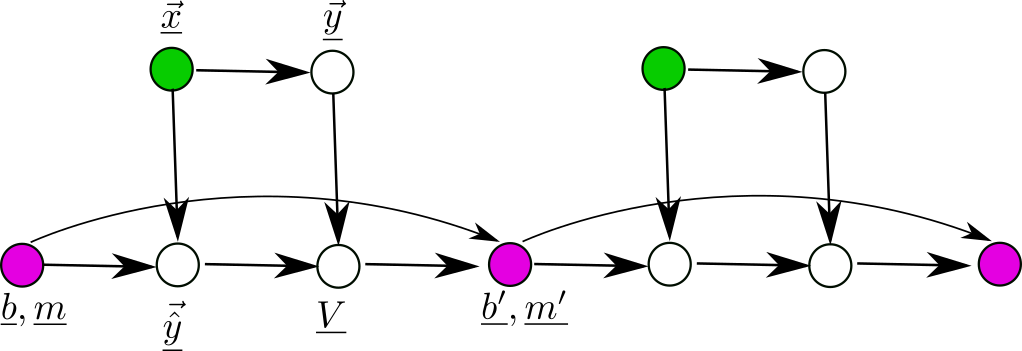
\includegraphics[width=5in]{linreg/linreg.png}
\caption{Linear Regression} 
\label{fig-linreg}
\end{figure}

\begin{figure}[h!]
\centering
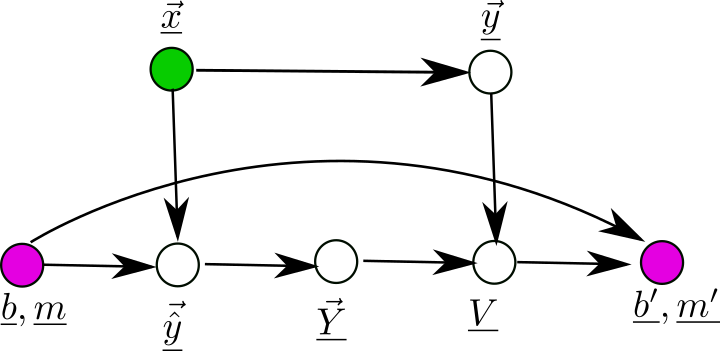
\includegraphics[width=3in]{linreg/linreg-emul.png}
\caption{B net of Fig.\ref{fig-linreg}  with new $\vec{\ul{Y}}$ node.}\label{fig-linreg-emul}
\end{figure}



Estimators $\hat{y}$ for linear and logistic regression.
\begin{itemize}
\item 

\textbf{Linear Regression:} $y\in \RR$. Note $\hat{y}\in \RR$. $(x,\hat{y}(x))$ is a straight line with y-intercept $b$ and slope $m$.
\beq
\hat{y}(x;b, m)= b + mx
\eeq

\item
\textbf{Logistic Regression:} $y\in\{0, 1\}$. Note $\hat{y}\in [0,1]$. $
(x,\hat{y}(x))$ is a sigmoid. Often in literature, $b,m$ are replaced by $\beta_0, \beta_1$. 
\beq
\hat{y}(x;b, m)=
\frac{1}{1+e^{-(b + m x)}}
\eeq
\end{itemize}

Define
\beq
V(b, m)=\sum_{x,y}P(x,y)| y-\hat{y}(x;b, m)|^2
\;.\label{eq-norm-cost}
\eeq
We want to minimize $V(b,m)$ (called a cost or loss function) wrt $b$ and $m$.


Node transition probabilities of B net of Fig.\ref{fig-linreg} given next in blue.

\beq\color{blue}
P(b,m) = \;{\rm given}
\eeq


\beq\color{blue}
P(\vecx)=\prod_i P(x[i])
\eeq

\beq\color{blue}
P(\vecy|\vecx)=\prod_i P(y[i]|x[i])
\eeq

\beq\color{blue}
P(\vec{\hat{y}}|\vecx, b, m)=\prod_i \delta(\hat{y}[i], \hat{y}(x[i],b,m))
\label{eq-replace1}
\eeq

\beq\color{blue}
P(V|\vec{\hat{y}}, \vecy)=
\delta(V, \frac{1}{nsam(\vecx)}\log \prod_i |\hat{y}[i]-y[i]|^2)
\label{eq-replace2}
\eeq
Let $\eta_b, \eta_m>0$. For $x=b,m$, if $x'-x=\Delta x = -\eta\frac{\partial V}{\partial x}$, then $\Delta V\approx \frac{-1}{\eta}(\Delta x)^2   \leq 0$ for $\eta>0$. This is called ``gradient descent".	
\beq\color{blue}
P(b'|V, b)=\delta(b', b-\eta_b\partial_b V)
\eeq
\beq\color{blue}
P(m'|V, m)=\delta(m', m-\eta_m\partial_m V)
\eeq


\begin{center}
\LARGE\textbf{{Generalization to $x$ with multiple components(features)}}
\end{center}
 Suppose that for each sample $i$, instead of $x[i]$ being a scalar, it has $n$ components called features:

 \beq
x[i] = (x_0[i], x_1[i], x_2[i] , \ldots x_{n-1}[i])
\;.\eeq

Slope $m$ is replaced by weights  

\beq
w = (w_0, w_1, w_3, , \ldots, w_{n-1})
\;,\eeq
and the product of 2  scalars $mx[i]$ is replaced by the inner vector product $w^Tx[i]$. 
\begin{center}
\LARGE\textbf{{Alternative $V(b,m)$ for logistic regression}} 
\end{center}
For logistic regression, since $y[i]\in \{0,1\}$ and $\hat{y}[i]\in [0,1]$ are both in the interval $[0,1]$, they can be interpreted as probabilities. Define 
probability distributions $p[i](x)$ and
$\hat{p}[i](x)$ for $x\in \{0,1\}$ by
\beq
p[i](1)=y[i],\;\;\; p[i](0)=1-y[i]
\eeq

\beq
\hat{p}[i](1)=\hat{y}[i],\;\;\; \hat{p}[i](0)=1-\hat{y}[i]
\eeq
Then for logistic regression, the following 2 cost functions $V(b,m)$
can be used as alternatives to the cost function Eq.(\ref{eq-norm-cost}) previously given.

\beq
V(b, m)= \frac{1}{nsam(\vecx)}\sum_i D_{KL}(p[i]\parallel \hat{p}[i])
\eeq

and

\beqa
V(b, m)&=&\frac{1}{nsam(\vecx)} \sum_i CE(p[i]\rarrow \hat{p}[i])\\
&=& \frac{-1}{nsam(\vecx)}\sum_i \left\{
y[i]\log \hat{y}[i] +
(1-y[i])\log (1- \hat{y}[i])\right\}\\
&=&
\frac{-1}{nsam(\vecx)}\sum_i 
\log \left\{\hat{y}[i]^{y[i]}(1- \hat{y}[i])^{(1-y[i])}\right\}\\
&=&
\frac{-1}{nsam(\vecx)}\sum_i 
\log P(\ul{Y}=y[i]|\hat{y}=\hat{y}[i])\\
&=&
-\sum_{x,y} P(x, y)
\log P(\ul{Y}=y|\hat{y}=\hat{y}(x,b,m))
\eeqa

Above, we used 
\beq
P(\ul{Y}=Y|\hat{y}) = \hat{y}^{Y}
[1-\hat{y}]^{1-Y}
\eeq
for $Y\in S_{\ul{Y}}=\{0,1\}$. (Bernoulli distribution).

There is no node corresponding to $\ul{Y}$
in the B net of Fig.\ref{fig-linreg}. Fig.\ref{fig-linreg-emul} shows a new B net that has a new node called $\vec{\ul{Y}}$ compared to the B net of Fig.\ref{fig-linreg}. One defines the transition probabilities for all nodes of Fig.\ref{fig-linreg-emul} except $\vec{\ul{Y}}$ and $\ul{V}$ the same as for Fig.\ref{fig-linreg}. For $\vec{\ul{Y}}$ and $\ul{V}$, one defines

\beq\color{blue}
P(Y[i]|\vec{\hat{y}})=
P(\ul{Y}=Y[i]|\hat{y}[i])
\eeq

\beq\color{blue}
P(V|\vec{Y}, \vecy)=
\delta(V, \frac{-1}{nsam(\vec{x})}\log \call)
\;,
\eeq
where $\call =\prod_i P(\ul{Y}=y[i]|\hat{y}[i] )$=likelihood.





%\printbibliography[heading=subbibliography]
%\end{refsection}

\end{document}	